\chapter{Accuracy tests and results}

Every test has been conducted with a camera positioned at 75 centimeters from the ground, with an inclination of 24.6 degrees. Furthermore, the webcam's field of view is approximatively 90 centimeters wide and almost 40 centimeters tall. QRCodes are placed on a 3x3 grid, in addition, their id is assigned from left to right and from the bottom to the top, as shown in figure \ref{field}.

\begin{figure}[hbt]
    \centering
    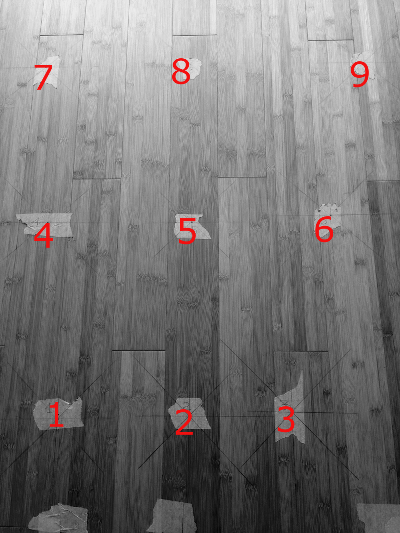
\includegraphics[scale=0.5]{img/field.png}
    \caption{QRCode's grid system. \label{field}}
\end{figure}

Moreover, in order to increase the number of tests using the same resources, three pictures for each angle was taken in every location. The orientations taken into account range from 0 to 360 degrees with an increment of 45 degrees in each step. Therefore, these tests was made on a basis of 216 pictures.
\newline
The positions of every marker was measured and they were hard-coded into the program in order to run the proposed software. As can be seen, Table \ref{qrpos} contains coordinates x and y in centimeters for every QRCode's id.

\begin{center}
	\label{qrpos}
  \begin{tabular}{ | l | l | l |}
    \hline
    id & pos\textunderscore x & pos\textunderscore y \\ \hline
    1 & 18.5 & 22 \\ \hline
    2 & 19 & 0 \\ \hline
    3 & 20 & -18 \\ \hline
    4 & 54 & 28 \\ \hline
    5 & 54 & 0 \\ \hline
    6 & 54 & -28 \\ \hline
    7 & 91 & 31 \\ \hline
    8 & 91 & 0 \\ \hline
    9 & 91 & -37 \\ \hline
  \end{tabular}
\end{center}